\documentclass[10pt,a4paper]{article}
\usepackage[utf8]{inputenc}
\usepackage[scale=0.7,vmarginratio={1:2},heightrounded]{geometry}

\usepackage[numbers]{natbib}

% link support in pdf
\usepackage[colorlinks,allcolors=blue,breaklinks = true]{hyperref}

% images in pdf
\usepackage{graphicx}
\graphicspath{{Bilder/}}
% multiple images
\usepackage{subfigure}
% images float in text
\usepackage{float}

% url support
\usepackage{url}
% glossarie support
\usepackage[acronym, automake]{glossaries}
\makeglossaries
\loadglsentries{glossary}

% math libs
\usepackage{amsmath}
\usepackage{amssymb}
\usepackage{amstext}
\usepackage{amsfonts}
\usepackage{mathrsfs}

% Code formating
\usepackage{listings}
\usepackage{color}

\definecolor{dkgreen}{rgb}{0,0.6,0}
\definecolor{gray}{rgb}{0.5,0.5,0.5}
\definecolor{mauve}{rgb}{0.58,0,0.82}

\lstset{frame=tb,
  language=Java,
  aboveskip=3mm,
  belowskip=3mm,
  showstringspaces=false,
  columns=flexible,
  basicstyle={\small\ttfamily},
  numbers=none,
  numberstyle=\tiny\color{gray},
  keywordstyle=\color{blue},
  commentstyle=\color{dkgreen},
  stringstyle=\color{mauve},
  breaklines=true,
  breakatwhitespace=true,
  tabsize=3
}

%Metadata
\title{TBD}
\author{Simon Hischier}
\date{April 2018}

\begin{document}

%Titlepage
\begin{titlepage}
%\maketitle
\centering
\vspace{1cm}
	{\scshape\LARGE Fachhochschule Luzern HSLU \par}
	\vspace{1cm}
	{\scshape\Large Studiengang Digital Ideation, Bachelor \par}
	
	{\scshape\Large 4. Semester\par}
	\vspace{1.5cm}
	{\huge\bf Procedural Generation in the age of AI\par}
	
	\vspace{10cm}
	{\Large Simon Hischier\par}
	\vfill

% Bottom of the page
	{\large \today\par}
\end{titlepage}

%Table of Contents Page
\renewcommand{\contentsname}{Inhalt}
\tableofcontents
\newpage

%First real page
\section{Abstract}
This work is juxtaposition between procedural generation with manually written algorithms and approaches with \gls{ml}. The question leading through this article therefore is: How does content creation in games differ between \gls{pcg} and \gls{ml} content creation? \gls{ml} and \gls{nn} are booming in big data and image recognition, only very few works address the artistic side like googles deep dream and this work takes a look at balancing procedural solutions and \gls{ml} solutions. The work first defines a few important terms and then lists different problemsolutions with procedural and with \gls{ml} examples. We defined the basic terms, discussed the desire to controll the artistic vision, worked through various examples for both approaches and listed possible solutions to some problems occuring with either procedural or \gls{ml} tasks. The goal of this work is to create awareness for creative \gls{ml} utilisation and to highlight challenges in both systems.

\section{Definitions}
\subsection{Procedural Content Generation}
The term \gls{pcg} defines a form of content generation that is automated. The content is created through algorithmic processes and with few to no human interaction. This allows for the creation of bigger, more random looking, unique content with less to no artist interaction.\cite{VanderLinden2014}

\subsection{Artificial Intelligence}
In 1956 the Book Automata Studies\cite{McCarthy1956} layed the ground work for \gls{ai} and the Dartmouth summer research project on artificial intelligence marked the key event "to nail the flag to the mast." McCarthy is credited for coining the phrase “artificial intelligence” and solidifying the orientation of the field\cite{moor2006dartmouth}. The name \gls{ai} was used ever since for various applications. Ever since this key event \gls{ai} is defined based on the goal that is tried to beeing achieved. Bernard Marr lists them as following:\cite{Marr2018}
\begin{enumerate}
\item Build systems that think exactly like humans do ("strong AI") 
\item Just get systems to work without figuring out how human reasoning works ("weak AI")
\item Use human reasoning as a model but not necessarily the end goal
\end{enumerate}
Marr referes with "strong AI" and "weak AI" to the paper written by John Searle where he defines a strong \gls{ai} of beeing able to think and have a mind and a weak \gls{ai} that can only act like it thinks and has a mind. The paper is also known for the "Chinese Room" argument\cite{Searle1980}. More terms for a \gls{ai} classification exist like Artificial General Intelligence (AGI) and the Artificial Superintelligence (ASI). These classifications are not further defined in this work.

Bernard Marr continues to list the various definitions for \gls{ai}. While the dictionaries list \gls{ai} as a definition, companies lack a clear definition and Marr extrapolates a definition from the companies research field. The dictionary definitions and his extrapolated definitions are listed here:
\begin{enumerate}
\item \textbf{The English Oxford Living Dictionary} "The theory and development of computer systems able to perform tasks normally requiring human intelligence, such as visual perception, speech recognition, decision making, and translation between languages."
\item \textbf{Merriam-Webster}
\begin{enumerate}
\item A branch of computer science dealing with the simulation of intelligent behavior in computers.
\item The capability of a machine to imitate intelligent human behavior.
\end{enumerate}
\item \textbf{The Encyclopedia Britannica} "artificial intelligence (AI), the ability of a digital computer or computer-controlled robot to perform tasks commonly associated with intelligent beings."
\item \textbf{Amazon} defines it as "the field of computer science dedicated to solving cognitive problems commonly associated with human intelligence, such as learning, problem solving, and pattern recognition."
\item \textbf{Google AI} "create smarter, more useful technology and help as many people as possible"
\item \textbf{Facebook AI Research} "advancing the file of machine intelligence and are creating new technologies to give people better ways to communicate."
\item \textbf{IBM}'s three areas of focus are "AI Engineering, building scalable AI models and tools; AI Tech where the core capabilities of AI such as natural language processing, speech and image recognition and reasoning are explored and AI Science, where expanding the frontiers of AI is the focus."\cite{Marr2018}
\end{enumerate}
This work is using the definition of the term \gls{ai} as listed in \textit{The Encyclopedia Britannica}. The fields described in this work can be categorized in the 3. objective listed by Marr "Use human reasoning as a model but not necessarily the end goal"\cite{Marr2018}

\subsection{The Difference between AI, Machinelearning, Deeplearning}
\label{sec:AIMachinelearningDeeplearning}
As shown before, \gls{ai} is not a new phenomena and even \gls{ml} is known for quite some time. There is not a great difference between \gls{ai}, \gls{ml} and deep learning. They are subsets of the previous. While \gls{ai} still is a very broad term \gls{ml} and deep learning are closer together. Deep learning introduces neuron simulation to \gls{ml} by creating discrete layers, connections and directions of data propagation\cite{MichaelCopeland2016}. The technology started to grow significantly around the year 2010. This seems to be related to the growing computational power and the immense amount of collected and stored data\cite{MichaelCopeland2016}. The illustration is showing the relationship between the 3 terms.
\begin{figure}[H]§
	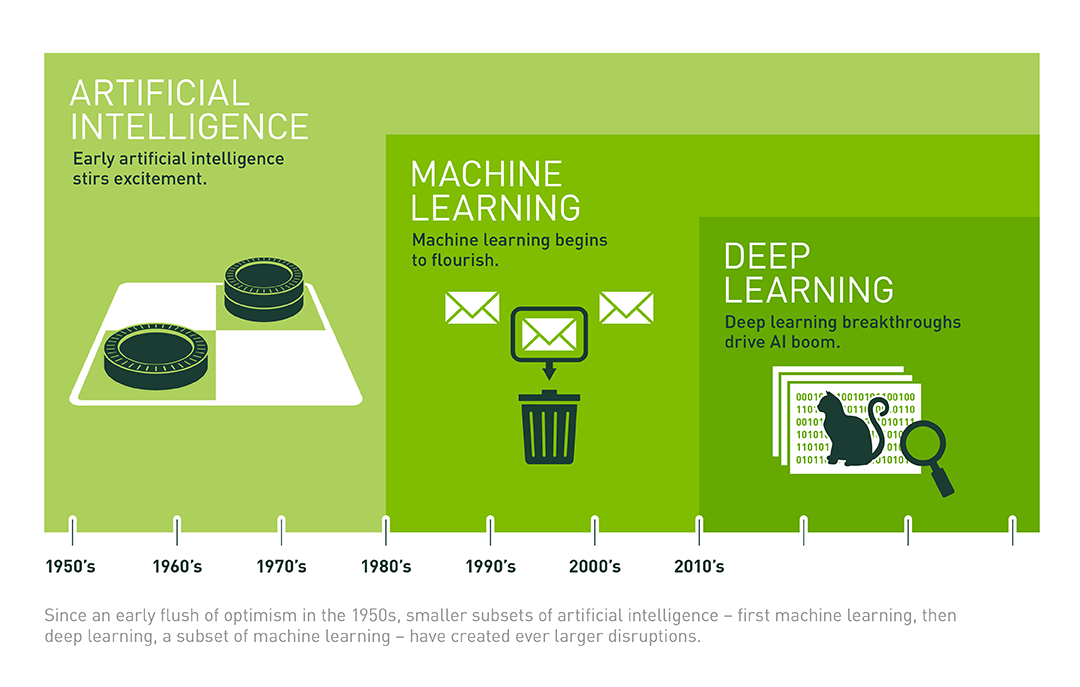
\includegraphics[width=\textwidth, height=\textheight, keepaspectratio]{Deep_Learning_Icons_R5.png}
	\caption{Levels of AI as Image\cite{MichaelCopeland2016}.}
\end{figure}

\subsection{Often used Neural Networks}
\subsubsection{Convolution Neural Network}
The \gls{cnn} describes a method to reduce input data and enhance \gls{nn} performance. The convolution allows for faster calculations and reduces memory requirements. This advantages make \gls{cnn} very desirable for image recognition and voice recognition tasks and are widely used in these fields.

\subsubsection{Recurrent Neural Networks}
As explained in \autoref{sec:AIMachinelearningDeeplearning} \gls{ml} is a broad term and includes a variety of models. The \gls{rnn} are networks for tasks where we need some kind of persistance. If we want to classify videoframes the network should have some kind of consistency.\cite{Olah2015} A network should persist the last seen data and not reclassify items every frame. Reclassifying without previous context could lead to different recognitions in every frame for the same object.

\subsubsection{Long short-term memory}
\gls{rnn} are good for persisting very recent information. Sentences are a great example: "Ships are built to float on \textit{water}". The \gls{rnn} is great in filling the end of this sentence. Problems arise when the information is needed a lot later. The more information is inbetween the contextual references the more unreiable a basic \gls{rnn} gets. Books for example can have references on the last page to the very beginning. For such tasks a \gls{lstm} model is the perfect fit. The \gls{lstm} network was introduced by Hochreiter Sepp and Urgen Schmidhuber\citep{Hochreiter1997}. A \gls{lstm} is a specialized version of a \gls{rnn} which is designed for these kind of tasks. Almost all \gls{rnn} tasks can be achieved with a \gls{lstm} \gls{rnn}\cite{Olah2015}.

\section{The artistic vision and the generation}\label{sec:visionVSgeneration}
Generating content for games is a fundamental artistic choice for game developers. The generation in various forms is linked to a decrease in the artistic vision. Designers have to step away from micro-controlling game parts like environment, shapes, colors, enemy behaviours etc. Therefore games do include \gls{pcg} in different ways and in various depths. Big studios tend to stick to more controlled experiences and have more (human-)resources to ensure this vision. We define a list of various depths of \gls{pcg}:
\begin{enumerate}
\item \textbf{No generation} (ex. \textit{Super Mario Bros} (Nintendo, 1985) where everything was handplaced, drawn and animated as explained in \textit{Super Mario Bros}. Level 1-1\cite{EurogamerMiyamotoInterview})
\item \textbf{Content generation in the game making phase.} (ex. \textit{The Elder Scrolls Oblivion} (Bethesda Softworks, 2006) used \gls{pcg} to generated most of the world before the artists curated it.\cite{PCGamerCarterInterview} An example of a widely used \gls{pcg} algorithm middleware for game studios is SpeedTree\cite{SpeedTree}
\item \textbf{Gameplay (partially) definded or influenced} by \gls{pcg} such as the sidequests for \textit{The Elder Scrolls Skyrim} (Bethesda Softworks, 2011) which were endlessly generated\cite{Bertz2011} or Castles in \textit{Rogue Legacy} (Cellar Door Games, 2013) which are generated procedurally but the game has some kind of continuosity and progress on top of the castle runs.\cite{Stanton2013}
\item \textbf{Games almost completely generated} ex. \textit{Dwarf Fortress} (Dwarf Fortress, 2006) doesn't stop at the map generation. It starts out generating the history of this world and everything that happened before.\cite{Champandard2012}
\end{enumerate}
Games and even game genres do fall into these different levels of \gls{pcg}. A major role for this classification of games and game genres is the depth of artistic control or lack therefore.\cite{VanderLinden2014} Games that do rely more on \gls{pcg} tend to focus more on the fun gameplay rather then an intriguing story and complex characters. Further categorization and different methods of \gls{pcg} can be found in the Paper from van der Linden, Lopes and Bidarra\cite{VanderLinden2014}.

\section{Procedural Content Generation and AI}
As explained in \hyperref[sec:visionVSgeneration]{The artistic vision and the generation} there are various genres and games falling into different levels of \gls{pcg}. Due to the type of gameplay and game mechanics linked to \gls{pcg}, games with high levels of procedural generation can easily be identified. We hope \gls{ai} blurs the line between \gls{pcg} and handcrafted more. A goal for \gls{ai} components is to create \gls{pcg} games that are less distinguishable from handcrafted counterparts. By extending the \gls{pcg} with \gls{ai} we hope to have a more natural and handcrafted feel to \gls{pcg} type games. As \gls{ml} gets used more in games, the applications starts to vary further.

\section{Applications of Procedural Approaches}
Procedural generation of content varies wildly and can affect most gameparts. In \hyperref[sec:visionVSgeneration]{The artistic vision and the generation} we made an attempt to categorize the different stages and depths of automation. However the reason to use \gls{pcg} can range from necessity (memory limitations, more content to create then time to create it) to artistic choice (pattern and style generation). The \gls{pcg} algorithms allow to shift the artists focus away from the detail work to broader concepts. An example might be the world biomes in \textit{Minecraft} (Markus Persson, 2009) instead of exact placements of blocks and levelparts. \gls{pcg} has multiple facettes and listing the different reasons to use \gls{pcg} is not feasable in this work. What all procedural algorithms share in common is a tradeoff between disk space and computing time. A big advantage of \gls{pcg} is the great influence on the outcome and the artists controll over what exactly gets generated. With \gls{pcg} algorithms the artist has complete controll over the process of generating the drawback for this is an increasing amount of programming work and complexity. Another interesting property of \gls{pcg} is the curiosity involved in finding out what the algorithm generated. Eventhough the artist has complete controll over \textbf{how} content is generated they don't controll \textbf{what} exactly is generated, leaving said room for curiosity. Some unsorted and randomly picked examples of \gls{pcg} widely used are listed below.

\subsection{Level Generation}
Procedural level generation is around for a very long time. It was present during the arcade games because of the need to possibly play endlessly to get the high score. It got carried over to the personal computer, generating dungeons to provide unique experiences\cite{VanderLinden2014} and to counter floppy disk memory limitations. Currently one of the most known level generators is used in \textit{Minecraft} (Markus Persson, 2009) where the endless worlds are used to feed the players curiosity. The strength of these systems is that worlds are replicable (see world-seeds in Minecraft), can be controlled and fine-tuned and don't necessarily need a lot of computational power. They are expandable, maintainable and errors in the level generation process can be checked and fixed. A drawback is the complexity (or lack therefore) of such generators. Worlds can look repetitive and empty.

\subsection{Text to Speech}
Procedural approaches of text to speech up until now were more on the functional side. Text to speech has great challenges and voices can sound very monotone, lack highlights and are in general not used in games. Games either hire voice actors to read the text examples or display the text as is.

\section{Applications of Neural Network systems}
In comparison to the procedural approach of extending the algorithm the \gls{nn} approach is a very top down approach. The \gls{nn} needs a lot of computing resources and a great set of datapoints. The user does not have to (neither can) finetune the parameters for the generation directly as is with the \gls{pcg}. The users can choose different \gls{nn} types and can only control the various \gls{ml} controllers which come with the \gls{nn}. There is no direct influence on the generation itself, the output can be changed by letting the \gls{ml} model guess and finetune its weights until it gets the desired outputs. This changes the workflow significantly and to use the network a user has to know what outcome is desired. This stands in direct opposition to procedural algorithms where the output is a result of the written code. With \gls{nn}s the artists decides on what the concept is which the \gls{nn} should learn and he then teaches the \gls{nn} to follow the concept. Testing such a \gls{nn} and evaluating corner cases is very labor intensive and debugging is not a real option. The big drawback when creating a new model is the need for existing data. The procedural algorithms can be programmed to work with a random number and data can optionally be fed into the algorithm to shape the outcome while developing. For a \gls{nn} to generate data in the desired way one has to first create a lot of examples that look like the desired outcome to train the network with. This is the biggest difference when working with \gls{nn} and procedural algorithms. To show a few examples of various \gls{nn} we list examples where the \gls{nn} \gls{ai} performs great. Note that the examples represent a small field of applications and the examples are randomly picked. This field is under extensive research and there are significant parts left out like image combination\cite{Luan2018}, style transfer, evolution of objects and many more.

\subsection{Face representation in games}
An area where \gls{ai} is much more effective then handwritten procedrual approaches is face reconstruction and face mapping. Webcam feeds have no depth information and creating 3D faces from photos is a laborintensive work. Actual research shows \gls{ml} is capable of reconstruction and position maping 3D avatars from single images. It's robust, fast and stable\cite{Feng2018}. A large area in the games industry is avatar faces. Massive Multiplayer Games tend to have elaborate avatar creaton tools to customize the game character. Games like \textit{Arma} (Bohemia Interactive, 2013) are using the users voice in multiplayer sessions and try to synchronize the avatars lips with the players spoken words. Online chats with avatar representations such as \textit{VRChat} (VRChat Inc., 2017) have immersive VR worlds where players can walk and talk in a virtual environment. For streaming platforms like \textit{Twitch} (Amazon, 2011) a webcam feed is part of the majority of streams. All these different games, genres and platforms would benefit from some kind of reconstruction of the players face. \textit(Arma) could have the real users faces represented in real-time in the game, non human avatars could use \gls{ai} to map the users lips and expressions on to the virtual avatars. Streamer could have their faces as 3D models or have an avatar instead of a live camera feed.

\subsection{text to speech}
Text is a big part of games. Extreme examples of games with word counts comparable to The Lord of the Rings book trilogy are present in the \gls{rpg} and text adventure genre. For this games voicing every line is out of range for game studios and therefore players have to read most of the text. With a trained \gls{nn} it is possible to have a voice actor read example texts and let the \gls{nn} generate the voice from the written text in the game\cite{Shen2017}. Although a demonstration used 24.6 hours of training data this number can probably be reduced. Another paper shows, that even singing can be generated with 16 and 35 minutes of sentences read out\cite{Blaauw2017}. The later audio example lengths could potentially open doors for further applications of text to speech such as online chat using the users voice to generate spoken words for the other users.

\subsection{Game AI}
Something almost all games have is computer players controlled by \gls{ai}. There are a variety of different solutions to mimic human behaviour. The more complex a game is the harder it is to write comprehensible game \gls{ai}. Games like Go remain too hard to calculate a winning strategy. There are simply too many complex situations and too many possible paths to explore. In this field \gls{ai} really showed its power and Alpha Go defeating the world champion was a major step in \gls{ai}\cite{Silver2016}\cite{Silver2017}. While Alpha Go did need more hardwarepower then the usual gaming computer provides, OpenAI demonstrated a less powerhungry \gls{ai} for \textit{Dota 2} (Valve Corporation, 2013). At the International Tournament 2017 OpenAI demonstrated an \gls{ai} that beat Pro Players at the game reliably.\cite{Openai2017} The rules were more strict then a normal game of Dota 2 but given enough time and resources, an \gls{ai} that can beat Professional teams is likely. These types of games are a big challenge to program computer players for because they allow for wacky situations, situations never seen before and asymmetric or incomplete information about the other players. A strong field for \gls{ml} is creating \gls{ai} that always remains and adapts to the level of the human player. This is almost impossible to program by hand or with other approaches.

\subsection{Anti-Cheating}
Valve demonstrated a very significant increase in Anti-Cheat software effectiveness after they started to use deep learning. Old methods of hardcoding different checks did and does only lead to an arms race with the cheat providers. The new approach requires the company to maintain a powerfull server. A big drawback is, that the company has to own a more powerfull \gls{nn} and have more complete information to not get outsmarted by cheat providers\cite{McDonald2018}.

\section{Level Generation compared}
Level generation can be done via \gls{ml} as shown by Adam Geitgey\citep{AdamGeitgey2016} or \gls{pcg} depending on the desired output. Both approaches could potentially be combined for a wider variety. What both approaches lack is the carefully curated and manually designed human aspect of levels. The amount of detail and teaching in a single \textit{Super Mario Bros.} (Nintendo, 1985) level\cite{EurogamerMiyamotoInterview} is still not feasible by both approaches.

\section{shortcomings of AI}
\textbf{TO DO}
, generation \gls{rpg}s started to rely more on generation and artists curation of content to fill the initial world.
-even more lack of control, very big input array
-same problems as with \gls{pcg} because a more complex understanding is needed for an artistic vision across levels

\section{Procedural Content Generation and Machine Learning}
\textbf{TO DO}
The different strengths of \gls{pcg} and \gls{ml} suggest, that \gls{ml} is an extension in the content generation toolbox rather then a replacement.

super mario level 1-1 teaching ...

\gls{ai} is a new type of content generation with overlapping areas to \gls{pcg} and classic game \gls{ai}s. It can go from a \gls{pcg} replacement to games revolving around an \gls{ai} (Alien game colonial marines?)

\section{Conclusion}

?
while pcg and ai both have very real and usefull ... they still lack the thought through creative possibilities possible by humans.
showed in the example of level generation how the different approaches are
ai is harder to controll then \gls{pcg} and depending on the area is a lot more labor intensive. But has fields where \gls{pcg} is inappropriate.
ai needs more calculation power, big initial work
know what to do upfront
?

\section{Referenzen und Akronyme}

\printglossaries

%\renewcommand{\refname}{myBibliography}
\bibliography{myBibliography}
%\bibliographystyle{unsrtnat}
%\bibliographystyle{plainnat}
\bibliographystyle{unsrt}
%\bibliography{myBibliography}

%list the figures and tables in contents
%\addcontentsline{toc}{section}{\listfigurename}
%\addcontentsline{toc}{section}{\listtablename}

%print list
\listoffigures
\listoftables

%\nocite{*}

\end{document}